\documentclass{article}

% Packages
\usepackage{amsmath}
\usepackage{pdfpages}
\usepackage{tikz}

\usepackage{float}
\usepackage{graphicx}
\graphicspath{ {./images/}}

\usepackage{setspace}
\setstretch{1.5}

% Configuring biblatex
\usepackage{biblatex}
\addbibresource{project_formulation/bib.bib}

% Configuring Fancy hdr
\usepackage{fancyhdr}
\pagestyle{fancy}

\fancyhead[R]{Bachelor Thesis}
\fancyhead[L]{Philip Oliver Mejer Jørgensen}

% Configuring title page
\title{\textbf{Detection of Vinyl Chloride in environmental water samples}~\\[5mm]
\large{By: Philip Oliver Mejer Jørgensen}~\\[5mm]

\includegraphics[width=0.4\textwidth]{sdulogo.png}}
\author{
Supervisors:~\\[3mm]
Main supervisor: Associate Professor Roana de Oliveira Hansen~\\[15mm]
University of Southern Denmark (SDU)\\
Faculty of Engineering - Mechatronics\\
Sønderborg, Denmark
}
\date{January 2024}

% Main document
\begin{document}
\maketitle
~\\[2mm]
\begin{center}
\large{
Thesis submitted\\
as a part of the\\
Bachelor of Engineering in Mechatronics
}
\end{center}
\thispagestyle{empty}
\newpage

\addcontentsline{toc}{section}{Abstract}
\begin{abstract}
Abstract. write toward the end
\end{abstract}

\listoffigures

\addcontentsline{toc}{section}{Abbreviations}
\section*{Abbreviations}
\begin{tabular}{ll}
VOC     & Volatile Organic Compound \\
VC      & Vinyl Chloride \\
PVC     & Polyvinyl Chloride \\
\end{tabular}
\newpage

\tableofcontents

\newpage

% The different sections to include:

\addcontentsline{toc}{section}{Project Formulation}
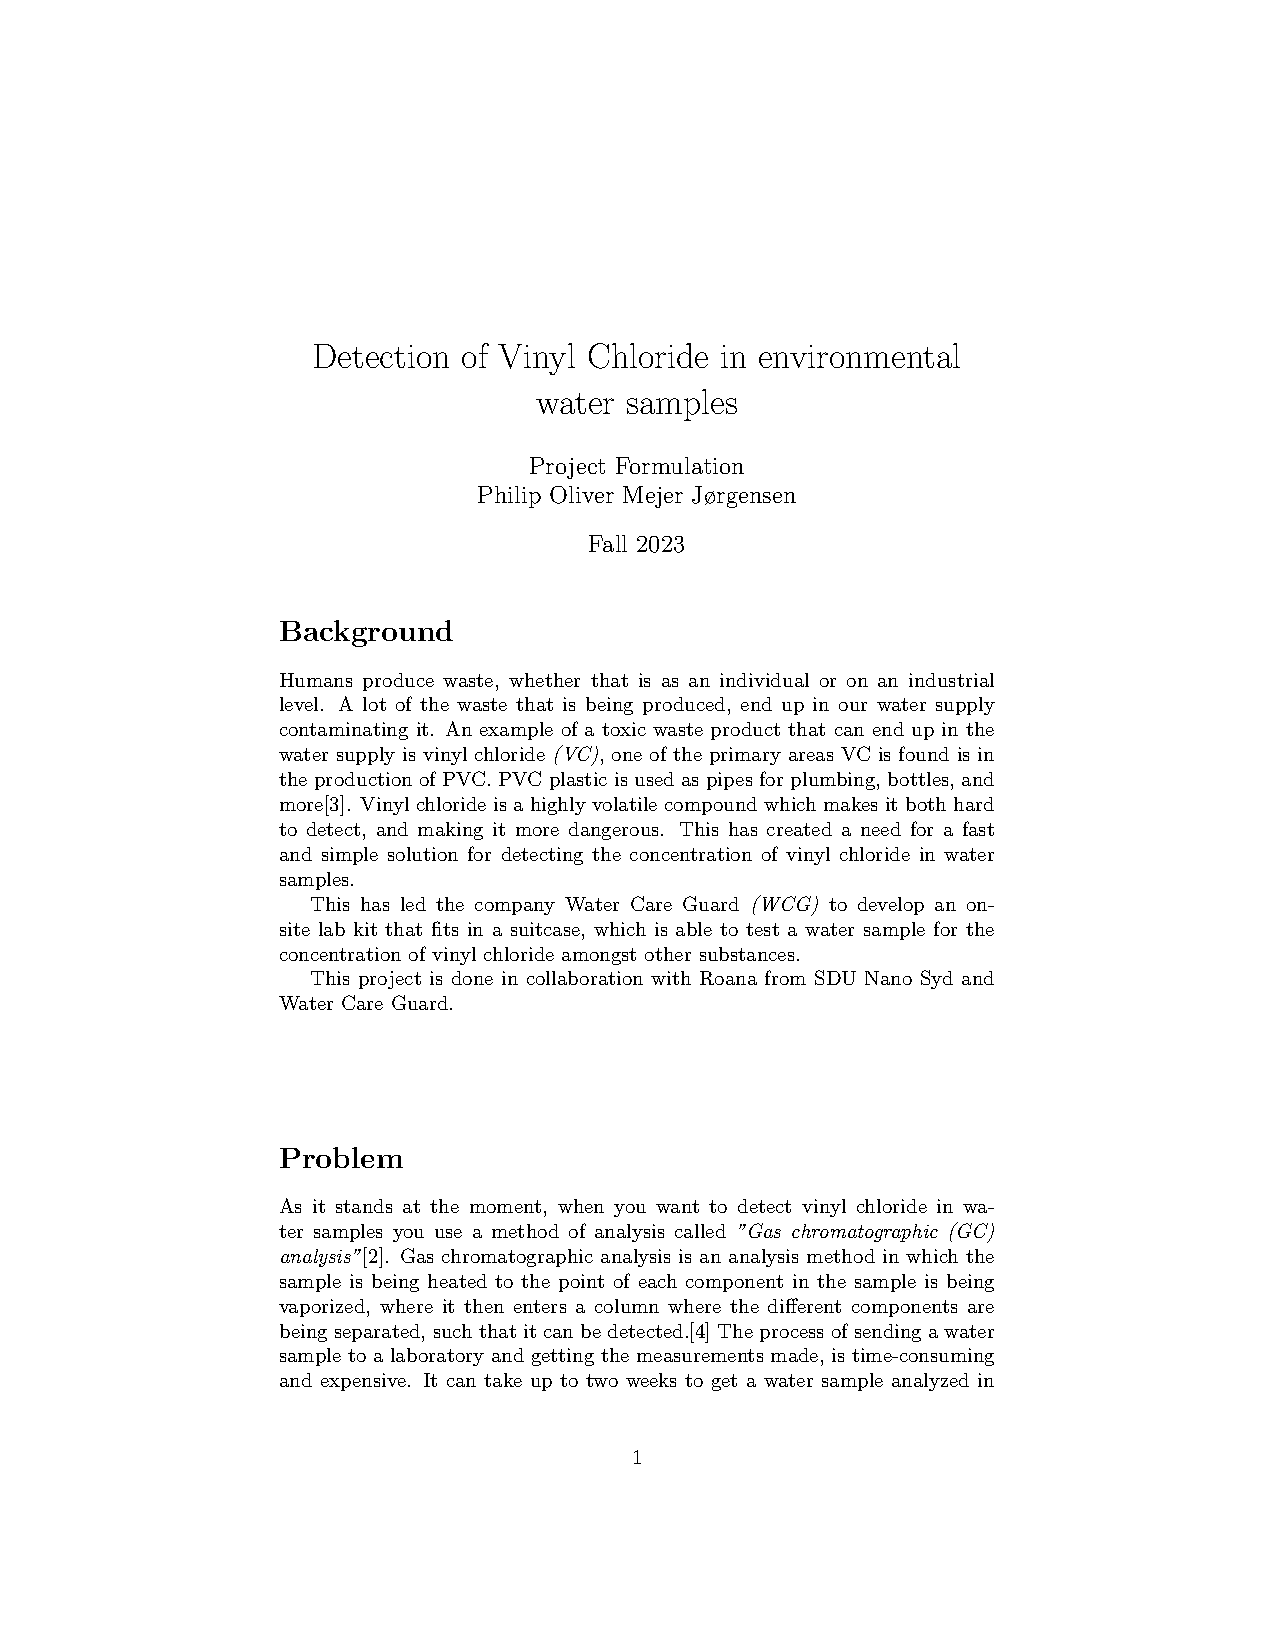
\includepdf[pages=-]{project_formulation/project_formulation.pdf}

\section{Introduction}
\subsection{Background}
Humans have been producing waste for a long time, but as the materials that we use change so has our waste.
In the early 20th century with the invention of fully synthetic plastic by the Belgian chemist Leo Baekeland in 1907\cite{plastic_history}, started a new type of anthropogenic pollution.
One type of plastic known as Polyvinyl Chloride (PVC), which was first synthesized in 1872 by Dr. Eugen Baumann\cite{pvc_origin}, it was first plastasized by Dr. Waldo L. Semon in 1926\cite{history_pvc}.
The introduction of plastics and especially PVC plastics, has introduced a new biproduct which is a highly toxic volatile organic compound (VOC), called Vinyl Chloride (VC).
Vinyl chloride is a biproduct in the production of PVC plastics, from it being used as the main component in the production of PVC plastics.
PVC plastics are used in a lot of different areas like construction piping, packaging, wires, toys, etc. in figure \ref{fig:pvc_applications} some examples of PVC applications are shown.

% Applications for PVC plastic figure
\begin{figure}[H]
    \centering
    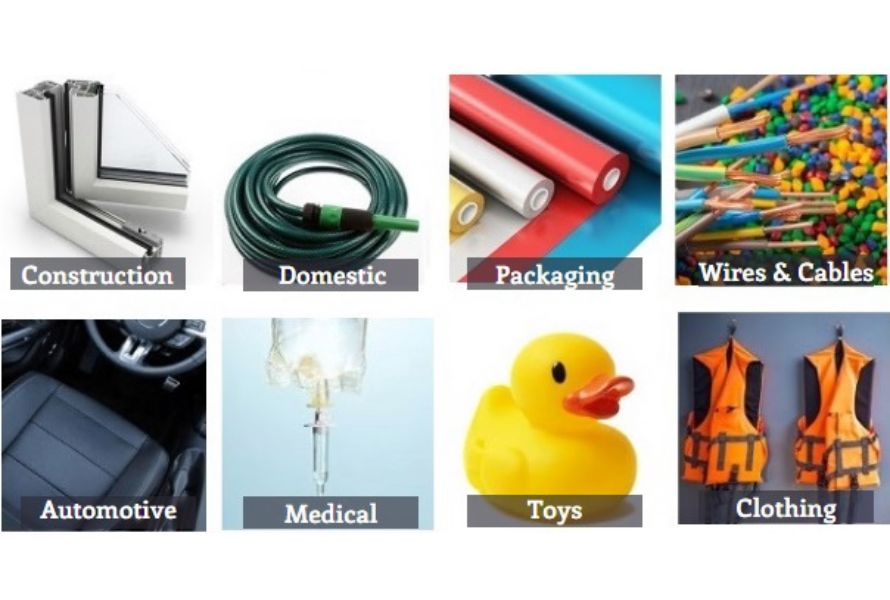
\includegraphics[width=0.7\textwidth]{pvc_applications.jpg}
    \caption{Applications for PVC plastic\cite{pvc_applications_euroeplas}}
    \label{fig:pvc_applications}
\end{figure}

People can be exposed to vinyl chloride in different ways, through inhalating contaminated air, contaminated water etc.
If vinyl chloride contaminate a water supply to a household, it can contaminate the air in the household leading to the inhabitants being exposed to vinyl chloride. \cite{vc_cancer}
One of the main dangers with exposure to vinyl chloride is the increased risk of cancer, and in particular liver cancer.\cite{vc_cancer}
In addition according to \textit{"kemibrug.dk"}\footnote{A database for information regarding chemicals}, vinyl chloride can also affect the central nervous system with symptoms like headache, dizziness, nausea and a possibility of loss of conscioiusness, as well as the inhalation the chemical is also easily absorbed through the skin which can lead to similar effects as of those from inhilation.\cite{vc_kemibrug}


At the moment the primary way to analyze whether there is vinyl chloride present in a water sample is through gas chromatogrpahy
test

\section{Theory}
\subsection{What is \textit{Refractive index}?}
\subsection{The photonic cystals, a tool for measuring the refractive index}

\newpage
\section{Building a database}
\subsection{Measuring vinyl chloride in a sample}
\subsubsection{General methodology}
\subsubsection{Measuring using the Water Care Guard suitcase}
\subsubsection{Measuring using the Shimadzu UV-1900 spectrophotometer}
\subsection{Problems}
\subsection{Data analysis}

\newpage
\section{User interface}
\subsection{API Interface}
\subsection{Graphical User Interface}

\newpage
\section{Conclusion}

\newpage

\printbibliography

\section{Appendix}
% Add the code here, and a flowchart version to describe the logic

\end{document}